\documentclass{article}
\usepackage{fullpage}
\usepackage{amsmath, amssymb}
\usepackage[hidelinks]{hyperref}
\usepackage[utf8]{inputenc}
\usepackage{natbib}
\usepackage{graphicx}
\usepackage{enumitem}
\bibliographystyle{plainnat}


\newcommand{\R}{\mathbb{R}}
\newcommand{\Q}{\mathbb{Q}}
\newcommand{\Z}{\mathbb{Z}}
\newcommand{\N}{\mathbb{N}}
\newcommand{\C}{\mathbb{C}}

\renewcommand{\P}{\mathbb{P}}
\newcommand{\E}{\mathbb{E}}
\newcommand{\var}{\mathop{\mbox{Var}}}
\newcommand{\cov}{\mathop{\mbox{cov}}}
%\newcommand{\det}{\mathop{\mbox{det}}}
\newcommand{\supp}{\mathop{\mbox{supp}}}
\newcommand{\sgn}{\mathop{\mbox{sgn}}}
\newcommand{\EE}[1]{\E\!\left[#1\right]}
\newcommand{\PP}[1]{\P\!\left\{#1\right\}}
\newcommand{\PPP}[2]{\P_{#1}\!\left\{#2\right\}}
\newcommand{\EEE}[2]{\E_{#1}\!\left[#2\right]}
\newcommand{\EEsup}[2]{\E^{#1}\!\left[#2\right]}

\newcommand{\bone}{\mathbf{1}}

\newcommand{\nodes}{\mathcal{N}}
\newcommand{\edges}{\mathcal{E}}
\newcommand{\sites}{\mathcal{S}}
\newcommand{\mutations}{\mathcal{M}}


\newcommand{\msprime}{\texttt{msprime}}

\usepackage{color}
\newcommand{\plr}[1]{{\em \color{blue} #1}}

\begin{document}

\title{Efficient forwards-time simulation with ancestral recombination graphs}
\author{Jerome Kelleher, 
        Jaime Ashander, and
        Peter L. Ralph}
\maketitle


\begin{abstract}
Coalescent simulations are very helpful but require random mating and neutrality.
For continuous space, polygenic selection, or detailed dissection of life history, 
we must use forwards-time, individual-based simulation.
These are much slower due in part to carrying around neutral genotypes irrelevant to the process.
Here we show how to efficiently produce and store the entire history of ancestry and recombination
(the ARG) from an individual-based simulation,
on which neutral mutations can be placed afterwards.
This has the promise of making large-scale, whole-genome simulations with realistic geography and selection finally possible.
\end{abstract}


%%%%%%%%%%%%%%%%%%%%%%
\section*{Introduction}

\plr{two main points below: can put down neutral mutations afterwards, and could be useful to compute stats even before that}

Since the 1980's, coalescent theory has enabled computer simulation of the results of population genetics models
identical to that which would be produced by large, randomly mating populations over long periods of time
without actually requiring simulation of so many generations or meioses.
Coalescent theory thus had three transformative effects on population genetics:
first, giving researchers better conceptual tools to describe \emph{gene trees} and thus bringing within-population trees into better focus;
second, producing analytical methods to estimate parameters of interest from genetic data (e.g. $\theta = 4N_e \mu$);
and finally, providing a computationally feasible method to produce computer simulations of population genetics processes.
However, these powerful advances came with substantial caveats:
the backwards-in-time processes that are described by coalescent theory
are only \emph{Markovian}, and thus feasible to work with,
thanks to the important assumptions of (a) random mating, and (b) neutrality.
\plr{Brief statement why this is.  Also include stationarity?}
Both assumptions can be side-stepped to a limited extent, and so coalescent methods are now commonly used to
simulate the results of population dynamics of a collection of randomly mating populations exchanging migrants,
having a small number of loci under selection.
Mapping results of such models onto real species can be challenging,
as these are often distributed across geographical space and may have large numbers of loci under various sorts of selection.
Furthermore, the relationship between the life history of a species --
fecundity and mortality schedules, allee effects, and demographic fluctuations --
are all absorbed into a single compound parameter, the coalescence rate.
These considerations, and increasing computational power, have led to a resurgence of interest in forwards-time, individual-based simulations.

With modern computing power, pure demographic calculations are not a barrier,
even though biological population sizes are often above $10^6$,
and coalescent theory tells us that a population of size $N$ 
must be run for a multiple of $N$ generations to produce stable genetic patterns.
However, if our interest lies in the resulting genetic patterns of variation
-- and often, the point of such simulations is to compare to real data --
then such simulations must somehow produce at the end data for each individual on a genomic scale.
As samples of most species genomes harbor tens or hundreds of millions of variant sites,
naively carrying full genotypes for even modest numbers of individuals through a simluation becomes quickly prohibitive.

However, it is thought that much of that variation is selectively neutral (or nearly so).
By definition, the alleles carried by individuals in a population at neutral sites
do not affect the population process.
For this reason, if one records the entire genealogical history of a population over the course of a simulation,
one can lay down neutral mutations on top of that history afterwards,
without loss of generality.
Precisely, we would need to know the genealogical tree relating all sampled individuals
at each position along the genome.

There is another compelling reason for recording the entire genealogical history.
In many applications, simulations are run for the purpose of comparing summary statistics of the resulting genomes
to those computed from real data,
with the purpose of inferring demographic history or identifying regions under selection.
However, for the same reason that neutral mutations can be laid down afterwards on the sequence of genealogical trees resulting from a simulation,
any summary statistic of genetic variation can be expressed as a statistic of the distribution of genealogical trees along the genome,
with additional noise introduced by mutations.
For instance, mean pairwise sequence diversity, $\theta$,
is most easily thought of as an estimator of $2 \mu t_{TMRCA}$, the mean time to most recent common ancestor
multiplied by twice the mutation rate,
with a relative error that is independent of the actual $t_{TMRCA}$.
As additional measurement noise makes simulation-based inference methods such as ABC or trained classifiers more diffcult,
it could be beneficial to compare the statistics observed in the data
to their expected values conditioned on the genealogical history,
as remaining mutational noise is not informative.
\plr{Say better.  A quick way to demonstrate this point?}

There is an obvious cost to recording all of history from a simulation,
rather than just the current state.
In this paper, we show how to use algorithmic tools and data structures developed for the coalescent simulator \msprime
to efficiently record, and later process, this history.

\plr{Quick review of the ARG and discussion of whether the ARG means the data structure or the reverse-time markov process (the former).}

%%%%%%%%%%%%%%%%%%%%%%
\section*{Methods}

\plr{Description of what we actually need to know in the end (the trees).}

\plr{Quick review of \msprime methods: sparse trees, tree differences.}

\plr{Specification for tables of nodes, edgesets, sites, and mutations (migrations?).}
\plr{Calling a collection of unordered tables a ``relaxed'' tree sequence
    but will make it clear that to do anything with these must sort first.}

\begin{itemize}
    \item[Nodes:]
        (flags, population, time)
    \item[Edgesets:]
        (left,  right,  parent,  children)
    \item[Sites:]
        (position,  ancestral\_state)
    \item[Mutations:]
        (site,  node,  derived\_state)
    \item \plr{Migrations?}
\end{itemize}


\plr{Steps to record information in forwards time.}
In the forwards simulation,
we record the results of each meiosis --
for each distinctly inherited segment of offspring chromosome,
we record the parental chromosome,
the left and right endpoints,
and the identities of any new mutations that have occurred on it.
This is recorded easily, without further processing,
in the relaxed tree sequence format.

Concretely, this is done as follows.
Suppose that the forwards simulation algorithm labels (haploid) individuals by integers,
which we call ``input labels'', 
to distinguish them from the ``node IDs'' given to these same individuals in the (output) tree sequence.
The algorithm maintains at all times a set of tables $(\nodes, \edgesets, \sites, \mutations)$
that record a relaxed tree sequence,
and an associative array $L$ that maps input labels to output node IDs, so that if $x$ is an input label,
then $L[x]$ is the corresponding output node ID.
We also always maintain $n$ to be the number of rows currently in the node table,
(so that with zero-indexed IDs, the next to be added will have node ID $n$),
$T_0$ to be the time of last simplification,
and $n_0$ the number of rows in the node table at that time. 

Initially, we begin with $n$ and $n_0$ equal to the number of rows in the initial node table,
and $L[j] = i_j$ for each $0 \le j < N$ if the initial input generation is labeled
$i_0$, \ldots, $i_{N-1}$.

At a reproduction event where haploid parents $x$ and $y$ produce offspring $u$ 
at time $t$ in population $p$,
\begin{enumerate}
    \item add a 
        $(
        \text{flags}=0,
        \text{population}=p, 
        \text{time}=t)$ row to the node table,
    \item set $L[u] = n$,
    \item and increment $n\mathrel{+}=1$.
\end{enumerate}
Then, for each interval $[\ell,r)$ that $u$ inherits from parent $z$
(where $z$ is either $x$ or $y$),
\begin{enumerate}[resume]
    \item add a 
        $( \text{left}=\ell,
        \text{right}=r, 
        \text{parent}=z, 
        \text{children}=(u,))$ row to the edgeset table.
\end{enumerate}
If furthermore there have been mutations at genomic locations $s_1$, \ldots, $s_k$
on this interval,
with derived states $q_1$, \ldots, $q_k$,
then for each $1 \le j \le k$,
\begin{enumerate}[resume]
    \item if $s_j$ is not in the site table, add a row
        $( \text{position}=s_j,
        \text{ancestral\_state}=0)$,
    \item find the site index $i$ whose position is $s_j$,
    \item and add a row
        $( \text{site}=i$,
           \text{node}=u$,
        \text{derived\_state}=q_j)$ to the mutation table.
\end{enumerate}

To \textbf{simplify} the tree sequence at time $T$,
\begin{enumerate}
    \item add $T-T_0$ to each time in the first $n_0$ rows of the node table,
        and replace each remaining time $t$ with $T-t$.
\end{enumerate}
Then, pass the set of currently alive input IDs,
$i_0, \ldots, i_{N-1}$ to the simplificaiton algorithm,
which produces a tree sequence that has node ID $j$ corresponding to input ID $i_j$
for $0 \le j < N$, and
\begin{enumerate}[resume]
    \item empty $L$,
    \item let $L[j] = i_j$ for $0 \le j < N$,
    \item set $n$ to be the number of nodes in the new tree sequence and set $n_0 = n$, and finally
    \item set $T_0 = T$.
\end{enumerate}

Simplification keeps the tables to a managable size.
Since the map $L$ is updated to maintain the association between individuals in the simulation
and nodes in the tree sequence, simplification can be run regularly, 
as the simulation progresses.


\begin{figure}
    \begin{center}
        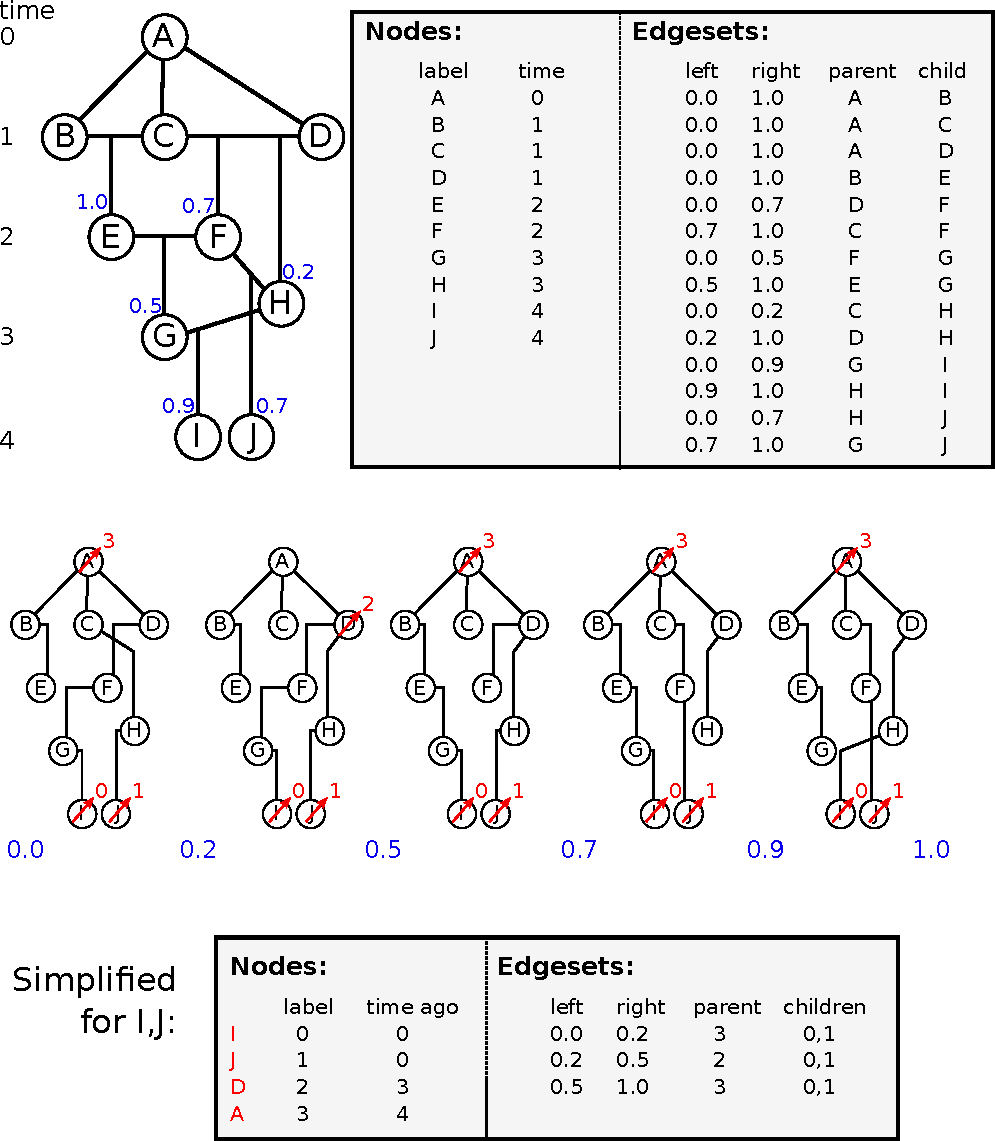
\includegraphics{method_diagram}
    \end{center}
    \caption{
        A simple example of the method.
        \textbf{Top:} the ARG shown on the left relates ten haploid individuals to each other.
        It is recorded, in forwards time, 
        in 10 node records (one for each individual)
        and 14 edgeset records (one for each distinctly inherited segment).
        Blue numbers denote crossing over locations in each meiosis.
        The individuals $B$, $C$, and $D$ inherit clonally from $A$
        to ensure rootnedness of resulting tree.
        \textbf{Center:} the five distinct trees relating all individuals to each other
        found across the chromosome (blue numbers denote locations on the chromosome).
        Labels after simplification are shown in red.
        \textbf{Bottom:} tables recording the tree sequence after simplification 
        with nodes $I$ and $J$ as samples.
        The mapping from labels in the forwards time simulation to nodes in the tree sequence
        is shown in red,
        which allows additional records to be added as the simulation progresses.
        \label{fig:method_diagram}
    }
\end{figure}

\plr{Something about simplification (but not the actual algorithm)
and estimates of how much memory usage is reduced by each time it is carried out.}
The resulting tables encode everything we need to know --
in fact, they record all of history for everyone alive at any time through the simulation.
This is much more than we need to reconstruct the genealogies and sequences
of a smaller sample of indidivuals.
Reducing this larger tree sequence to a smaller one relevant to a given set of ``sample'' nodes
we call \emph{simplification}.
Roughly, this works by tracing ancestry from the samples backwards through the recorded history,
adding node and edgeset records to the output only when coalescent events are reached.
This works exactly as in \msprime, allowing substantial re-use of algorithms;
the main difference being that parental choice, mutations, and recombination locations 
are determined by the input tree sequence
rather than randomly generated.
An example is shown in Figure \ref{fig:method_diagram}.
\plr{(trying to make the point strongly in the figure, that everything can be stored quite concisely)}

\plr{Note that you can begin the forwards-time simulation with the results of a previous (coalescent) one,
which is helpful so you don't need to run for so long (cite Wilkins).}
In this scheme,
at any point in the simulation genealogical history is recorded in a tree sequence.
This has two additional advantages.
First, simplification can be run periodically through the simulation,
taking the set of samples to be the entire currently alive population.
This is important as it keeps memory usage from growing linearly (and quickly) with time.
Second, the simulation can be \emph{begun} with a tree sequence produced by some other method --
for instance, by a coalescent simulation with \msprime.
This allows for incorporation of deep-time history beyond the reach of individual-based simulations.
Since geographic structure from times longer ago than the mixing time of migration across the range
has limited effect on modern genealogies \citep{wilkins_separation}
(other than possibly changing effective population size \citet{durretspatial}),
this may not negatively affect realism.

\plr{Something about putting mutations down on the tree sequence.}

\plr{Quick overview of how to efficiently hook this up with other code.}

%%%%%%%%%%%%%%%%%%%%%%
\section*{Results}

\plr{Estimates of run-time complexity}
Suppose that we wish to run a forwards-time simulation of $N$ individuals for $T$ generations,
in which there are $S$ selected loci and $L$ neutral loci.
We will estimate run-time complexity and memory usage for both a ``naive'' strategy that carries along neutral loci
and an ``ancestry-tracking'' strategy like that we consider here.
To do this, we assume that each individual must carry along its entire genotype.
More advanced schemes are used in some simulators,
but these increase efficiency by utilizing redundancy introduced by shared ancestry, 
which is effectively an intermediate scheme.
We omit the cost of computing a fitness function.

Both schemes must choose mates and recombination breakpoints,
and pass on selected genotypes.
The difference between the two comes from the tradeoff between
(a) passing on neutral genotypes, and
(b) recording and simplifying the tree sequence, and adding neutral genotypes afterwards.
(We assume here that selected genotypes are stored in the same way for both.)
Passing on neutral genotypes naively records $L$ items per individual each generation, discarding the previous generation.
\plr{do this better with numbers from nodes, edgesets}
Recording a tree sequence stores 2 parents and $\rho$ breakpoints on average each generation;
after $T$ generations this grows to $N \times T \times (2 + \rho)$ stored items.
However, after simplification a tree sequence for all $N$ individuals
only takes of order $N + \rho \log N$ records.
Simplification requires processing each of the initial records -- so, order of $N \times T \times \rho$ operations;


\begin{table}
\begin{center}
    \begin{tabular}{l||r|r||r|r|}
                    & \multicolumn{2}{|c|}{naive} & \multicolumn{2}{|c|}{ancestry-tracking} \\
                    & operations  & memory & operations  & memory \\
        mate choice & $N$       &   --  &   $N$     & -- \\
        recombination & $N\rho$ &   --  &   $N\rho$ & -- \\
    \end{tabular}
\end{center}
\end{table}

Comparison of simulation with/without msprime, using simuPOP 
or maybe just a simple haploid simulation with 1000 QTL and stabilizing selection on a trait (say).

Maybe an estimate of how long \emph{just} the ARG recording and simplification takes,
so that then we can say how fast the simulator would have to be to do $10^6$ whole chromosomes for $10^7$ generations
in a day.

%%%%%%%%%%%%%%%%%%%%%%
\section*{Conclusion}

This is a general-purpose strategy that can be applied to other methods.

All sorts of good reasons to want to have whole-genome simulations.

%%%%%%%%%%%%%%%%%%%%%%
\section*{Acknowledgements}

Kevin 

\bibliography{references}  

\end{document}
